\chapter{Literatuurstudie}
\label{chap:literatuurstudie}
In dit hoofdstuk wordt gestart met het bekijken welke mobiele apparaten er allemaal bestaan (\ref{sec:mobiele-apparaten}). 
Vervolgens wordt er gekeken wat er onder de motorkap van deze apparaten zit, namelijk welke mobiele besturingssystemen (\ref{sec:mobiele-besturingssystemen}), welke mobiele applicaties (\ref{sec:mobiele-applicaties}) en welke mobiele webbrowsers (\ref{sec:mobiele-webbrowsers}) er bestaan. 
Daarna komen de drie bouwblokken van het web aan bod (\ref{sec:html5-css3-js}), namelijk HTML, CSS en \js{}.
Hierna wordt ingegaan op bestaande mobiele HTML5-raamwerken (\ref{sec:mobiele-html5-raamwerken}).  
Ten slotte worden verschillende, reeds bestaande manieren om raamwerken te vergelijken, bekeken (\ref{sec:vergelijken-raamwerken}).

%%%%%%%%%%%%%%%%%%%%%%%%%%%%%%%%%%%%%%%%%%%%%%%%%%%%%%%%%%%%%%%%%%
%%%%%%%%%%%%%%%%%%%%%%%%%%%%%%%%%%%%%%%%%%%%%%%%%%%%%%%%%%%%%%%%%%

\section{Mobiele apparaten}
\label{sec:mobiele-apparaten}
Mobiele apparaten bestaan in alle soorten en maten, met weinig of veel opties, voor weinig of veel geld zoals wordt geïllustreerd op figuur \ref{fig:devices}. 
Het verdient daarom de aandacht om deze diversiteit onder de loep te nemen. 
Eerst wordt ingegaan op drie soorten mobiele apparaten, namelijk de smartphone, tablet en e-reader~\cite{GCF2013}.
Daarna wordt stilgestaan bij de kenmerken van deze apparaten~\cite{PhilDutson2012}.

\begin{figure}
  \centering
  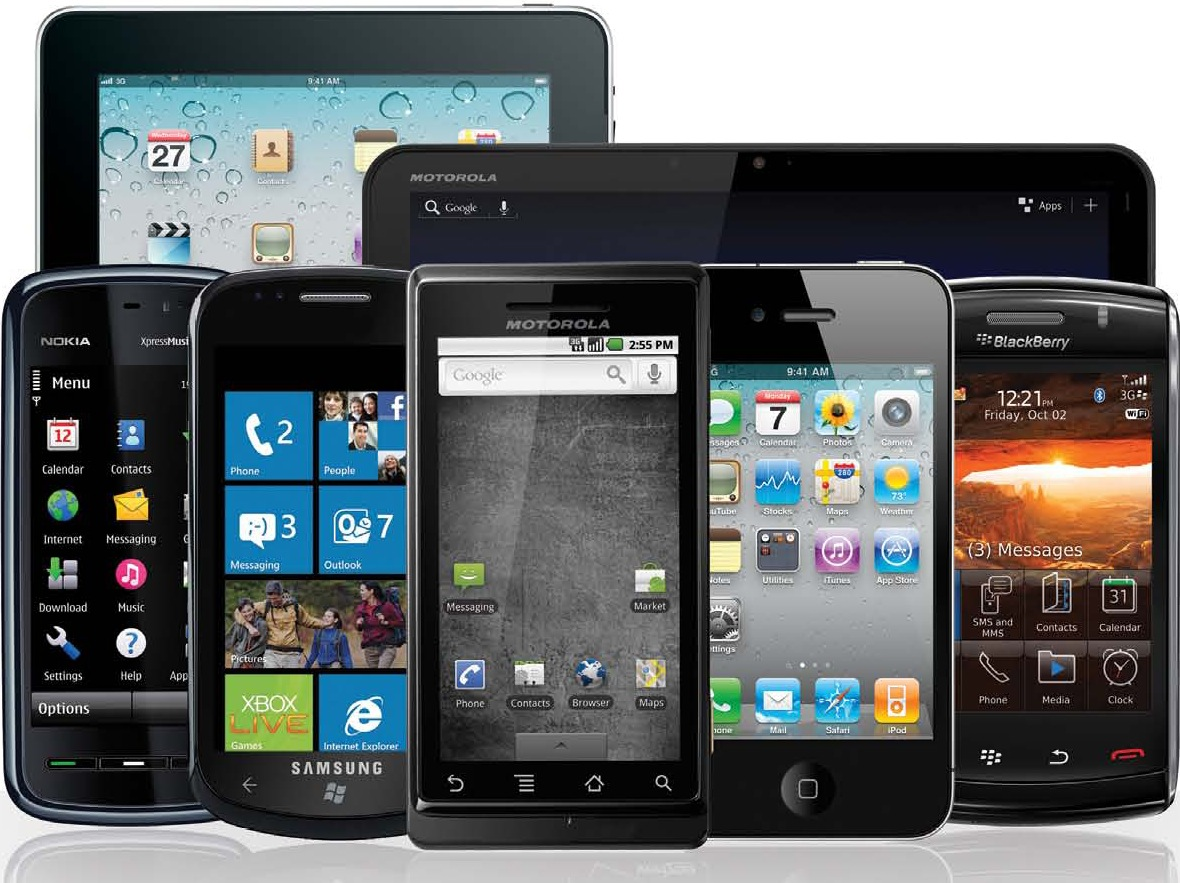
\includegraphics[height=0.6\textwidth]{figuren/mobile-devices.jpg}
  \caption{Verschillende mobiele apparaten~\cite{Grady2013}.}
  \label{fig:devices}
\end{figure}

\subsection{Soorten}
Sinds de voorstelling van de Apple iPhone in 2007~\cite{David2011}, stijgt het gebruik van de smartphone ontzettend snel in onze samenleving.  
Momenteel zijn er al meer dan 1 miljard smartphones in gebruik~\cite{Yang2012}. 
Dit zal tegen 2015 verdubbeld zijn~\cite{Gillett2012}.
Foto's of video's nemen, navigeren naar het dichtstbijzijnde restaurant of nog snel het weer voor de komende dagen opzoeken, het is allemaal mogelijk. 
Hoewel Apple de lat hoog heeft gelegd met het uitbrengen van de iPhone, zijn er ook nog andere spelers op de markt. 
Zo zijn er bijvoorbeeld de op Google's Android gebaseerde smartphones zoals de Nexus 4 en de op Windows Phone gebaseerde smartphones zoals de Nokia Lumia 800.

De tweede soort mobiele apparaten zijn tablets.
Tegen 2016 zulen er 760 miljoen tablets in gebruik zijn~\cite{Gillett2012}.
Ook hier kan terug gedacht worden aan één van Apple's succesvolle producten, namelijk de in 2010 uitgebrachte iPad~\cite{Apple2010}. 
Er dient echter wel opgemerkt te worden dat tien jaar voordien, Microsoft al eerder een tablet uitbracht met veel minder succes~\cite{Microsoft2000}.

%TODO voor sander: wat denk je er van om e-reader er uit smijten dan gewoon kort zeggen dat er nog PDA's, e-readers, enz bestaan? bij de kenmerken vertel ik toch enkel dingen over smartphone en tablet, dus die e-reader doet er niet echt toe..
De \term{e-reader} behoort tot de laatste categorie van mobiele apparaten. 
Deze wordt hoofdzakelijk gebruikt om digitale boeken te lezen, maar betere modellen laten bijvoorbeeld ook toe om te surfen op het Internet. 
Ook hier bestaat er een variëteit aan modellen zoals de Kindle van Amazon en de Reader van Sony.

\subsection{Kenmerken}
Door de vele verschillende soorten en modellen aan mobiele apparaten, is het nodig om op een hoog niveau te bekijken over welke kenmerken deze allemaal (kunnen) beschikken. 
Bij deze bespreking wordt ingegaan op de voornaamste kenmerken van smartphones en tablets. 
De kenmerken en tekst zijn gebaseerd op Phil Dutson~\cite{PhilDutson2012}.

\subsubsection{Resolutie en PPI}
Een eerste kenmerk waar vooral Apple met haar Retina graag mee uitpakt, is de resolutie. 
Dit is het aantal pixels getoond op het beeldscherm en wordt uitgedrukt in breedte $\times$ hoogte. 
Hoe kleiner, hoe minder er op het scherm kan worden getoond. 
Dit is vooral belangrijk wanneer veel informatie op het scherm wordt getoond. 
Bij een een kleine resolutie dient er gescrold te worden om te rest van de informatie te zien.
%Een overzicht van resoluties van bekende mobiele apparaten wordt getoond op de figuur \ref{fig:resoluties}.

Indien er naast de resolutie ook nog eens rekening wordt gehouden met de fysieke grootte van het scherm, wordt er gesproken over pixels per inch~(PPI). 
De eerste iPhone had een resolutie van 320$\times$480 en een 3,5” scherm, wat neerkomt op 163 PPI. 
De iPhone~4 (Retina) daarentegen heeft een resolutie van 640$\times$960 en een 3,5” scherm, wat neerkomt op 326 PPI. 
Met andere woorden zijn er meer pixels op dezelfde fysieke grootte geplaatst, wat een scherper beeld tot resultaat heeft. 

%TODO aan Sander: is deze afbeelding nuttig?  ik zou dan eerder een figuur met allemaal verschillende devices in mijn thesis steken dan een afbeelden met deze resoluties...
%\begin{figure}
%  \centering
%  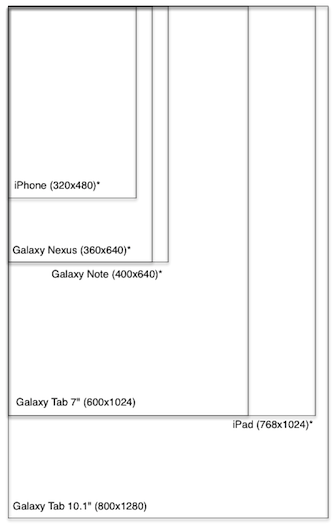
\includegraphics[height=0.8\textwidth]{figuren/mobile-devices-resolutions.png}
%  \caption{Resoluties van bekende mobiele apparaten~\cite{Wolfermann2012}.}
%  \label{fig:resoluties}
%\end{figure}

\subsubsection{Aanraakscherm}
De populaire soorten schermen zijn resistieve en capacitieve aanraakschermen. 
De eerstgenoemde soort maakt gebruik van twee lagen die gescheiden worden door een tussenruimte. 
Door druk ontstaat er contact tussen de twee lagen. 
Meestal wordt bij deze soort schermen een stylus meegeleverd. 

De laatstgenoemde soort maakt gebruik van veranderingen in frequentie. 
Door het scherm aan te raken met een vinger, dat een geleider is, ontstaat er een kleine verandering in frequentie die gedetecteerd wordt. 
Niet-geleidende materialen zullen geen frequentieverandering veroorzaken, wat verklaart dat zo'n scherm niet reageert als het wordt aangeraakt met een handschoen.

\subsubsection{Camera}
Praktisch ieder recent mobiele apparaat is uitgerust met een camera. 
Sommige bevatten zelfs twee camera's. 
De camera vooraan is veelal van mindere kwaliteit en wordt gebruikt om videogesprekken te voeren. 
Achteraan het apparaat zit dan een camera met hogere resolutie om foto's van betere kwaliteit te kunnen maken.

Twee voorbeelden van toepassingen van de camera zijn toegevoegde realiteit en het inscannen van barcodes.
Bij het eerstgenoemde wordt informatie toegevoegd aan het beeld dat door de camera wordt geregistreerd.
Het laatstgenoemde wordt gebruikt om de populaire QR-code in te scannen en te zien wat ze betekent.
Zo'n code kan tekst bevatten, een link naar een website, een telefoonnummer, enzovoort. 

\subsubsection{Verbinding}
Iedereen wil zoveel mogelijk met elkaar en het Internet verbonden zijn en dit kan ook op mobiele apparaten. 
Enerzijds kan gebruik worden gemaakt van mobiel Internet en anderzijds van draadloos Internet.
Daarnaast kan data ook uitgewisseld worden tussen apparaten, zonder hiervoor het Internet te gebruiken.
Een voorbeeld hiervan is Bluetooth dat een draadloze verbinding op korte afstand opzet.

\paragraph{Mobiel Internet}
Om dit in perspectief te plaatsen wordt eerst even teruggegaan in de tijd van mobiele communicatie.
Helemaal in het begin was er 1G, de eerste generatie mobiele telefonie, waarbij gesprekken analoog werd verzonden.
2G gebruikte daarentegen een digitaal netwerk, waarbij nieuwe diensten zoals SMS tekstberichten beschikbaar werden~\cite{Miami2008}.

Op de overgang van 2G naar 3G worden General Packet Radio Service~(GPRS) en Enhanced Data Rates for GSM Evolution~(EGDE) geplaatst.
GPRS is een uitbereiding op 2G waarbij data over het mobiele netwerk kan worden uitgewisseld.
De gebruiker moet slechts één maal inbellen op het netwerk en blijft daarna altijd verbonden.
Omdat niet alle telecomproviders hun hardware wilden aanpassen naar 3G, gebruikten ze EGDE dat een uitbreiding is op GPRS en grotere snelheden mogelijk maakt~\cite{Lauwers2007}.

3G maakt gebruikt van een volledige nieuwe technologie, namelijk Universal Mobile Telecommunications System~(UTMS).
Het is dus niet langer een uitbreiding op het bestaande netwerk zoals dat voor GPRS het geval was.
De vraag naar bandbreedte blijft, waardoor High-Speed Downlink Packet Access~(HSDPA) werd ontwikkeld. 
Het is een nieuwe implementatie van UTMS dat nog grotere snelheden toelaat~\cite{Lauwers2007}.

Op dit moment zijn telecomoperatoren volop bezig met de uitrol van 4G.
Dit moet nog grotere snelheden mogelijk maken door gebruik te maken van LTE Advanced, een verbetering van Long Term Evolution~(LTE).

\paragraph{Draadloos Internet}
Net zoals laptops draadloos verbinden met Internet via Wifi, kan dit ook op mobiele apparaten.
Vaak is de kost van mobiel Internet groter dan die van draadloos Internet, waardoor dit type van verbinding de voorkeur krijgt.

\subsubsection{GPS}
Met het \term{global positioning system} (GPS) kan de gebruiker zijn locatie opvragen en doorgeven aan een applicatie om zo bijvoorbeeld het dichtstbijzijnde restaurant te vinden. 
Doordat het wat kan duren vooraleer de locatie is vastgesteld via GPS, kan het mobiel apparaat ook gebruik maken van mobiele masten of het Internet om zo, hetzij minder nauwkeurig, sneller de locatie te bepalen.

%%%%%%%%%%%%%%%%%%%%%%%%%%%%%%%%%%%%%%%%%%%%%%%%%%%%%%%%%%%%%%%%%%
%%%%%%%%%%%%%%%%%%%%%%%%%%%%%%%%%%%%%%%%%%%%%%%%%%%%%%%%%%%%%%%%%%

\section{Mobiele besturingssystemen}
\label{sec:mobiele-besturingssystemen}
Net zoals er brede waaier bestaat aan besturingssystemen voor computers, geldt dit ook zo voor mobiele apparaten. 
In deze sectie wordt een overzicht gegeven van mobiele besturingssystemen met een significant marktaandeel~\cite{David2011, Hales2012} zoals iOS en Android, maar ook een nieuwkomer op de markt, namelijk Windows Phone.
iOS en Android haalden respectievelijk 14,9\% and 75,0\% in het derde kwartaal van 2012.
Windows Phone haalt 2\% van het marktaandeel binnen in datzelfde kwartaal~\cite{Protalinski2012}.

Bij ieder besturingssysteem zal ook over de winkel gepraat worden waar applicaties kunnen worden gevonden.
Net zoals programma's geïnstalleerd worden op een computer, kan dit ook voor mobiele apparaten.
Deze aangeboden applicaties worden verzameld in een winkel waarna de gebruiker ze, al dat niet gratis, kan downloaden en installeren.
De winkel kan de kwaliteit van deze applicaties hoog houden door regels op te leggen aan de ontwikkelaars (zie \ref{sec:mobiele-applicaties}).

\begin{table}[t]
\centering
\pgfplotstabletypeset[
  begin table=\begin{tabular}{l l},
  end table=\end{tabular},
  col sep=comma,
  header=true,
  string type,
  skip coltypes=true,
  columns={Versie,Marktaandeel},
  columns/Versie/.style={column name=\textbf{iOS}},  
  columns/Marktaandeel/.style={column name=\textbf{Marktaandeel (\%)}},
  every head row/.style={
    before row=\toprule,
    after row=\midrule},
  every last row/.style={
    after row=\bottomrule}
]{tabellen/ios.csv}
\quad
\pgfplotstabletypeset[
  begin table=\begin{tabular}{l l},
  end table=\end{tabular},
  col sep=comma,
  header=true,
  string type,
  skip coltypes=true,
  columns={Versie,Marktaandeel},
  columns/Versie/.style={column name=\textbf{Android}},  
  columns/Marktaandeel/.style={column name=\textbf{Marktaandeel (\%)}},
  every head row/.style={
    before row=\toprule,
    after row=\midrule},
  every last row/.style={
    after row=\bottomrule}
]{tabellen/android.csv}
\caption{Marktaandeel van iOS-versies op 8 mei 2013 en Android-versies op 1 mei 2013.  \protect\cite{Smith2013,Android2013}.}
\label{tabel:marktaandeel-ios-android}
\end{table}

\subsection{iOS}
Het iPhone-besturingssysteem is voor het eerst uitgekomen in juni 2007 tezamen met de iPhone. 
Later werd het hernoemd naar iPhone OS en uiteindelijk werd het iOS. 
Het is duidelijk dat iOS gebonden is aan de hardware van Apple. 
Verschillende versies volgden elkaar op: iOS 2 (juli 2008), iOS 3 (juni 2009), iOS 4 (juni 2010) en iOS 5 (oktober 2011)~\cite{Deitel2012, PhilDutson2012}. 

De nieuwste versie, iOS 6, werd uitgegeven in september 2012. 
Voorbeelden van nieuwigheden zijn de sterkere integratie van sociale media zoals \fb{} en Twitter en het gebruik van spraakcommando's~\cite{Deitel2012}. 
Op tabel \ref{tabel:marktaandeel-ios-android} is te zien dat drie vierde van de iOS-gebruikers al iOS 6 gebruikt.

Browsen op het web gebeurt met de geïnstalleerde Mobile Safari webbrowser (zie \ref{sec:mobile-safari}). Applicaties kunnen gedownload worden in winkel genaamd App Store, die sinds iOS 2 aanwezig is~\cite{Deitel2012}. 
Op deze winkel is er sterkte controle op de kwaliteit van de aangeboden applicaties door de ontwikkelaars zeer strikte regels op te leggen~\cite{Apple2010a}.

\subsection{Android}
Android Inc. werd opgericht in 2003 en werd in 2005 overgekocht door Google Inc~\cite{Satyesh2012}. 
Het is net zoals iOS een mobiel besturingssysteem, maar in tegenstelling tot iOS is het open~\cite{David2011}. 
De eerste stabiele versie, Android~1.0, kwam uit in september 2008. 
Ook hier volgden verschillende versies elkaar op: Android~2.0 (oktober 2009), Android~3.0 (februari 2011) en Android~4.0 (oktober 2011)~\cite{Satyesh2012}. 
Hun nieuwste versie, Android~4.2, werd aangekondigd in oktober 2012~\cite{Sawers2012}. 

Op tabel \ref{tabel:marktaandeel-ios-android} is het marktaandeel te zien van de verschillende Android-versies, waargenomen over een periode van 14 dagen. 
Het is duidelijk dat Gingerbread~(Android~2.3) bijna de helft van het marktaandeel inneemt.
Applicaties worden gedownload in de winkel genaamd Google Play. 
De controle op de kwaliteit van de aangeboden applicaties is minder strikt dan die van Apple.
De applicatie moeten aan een aantal algemene regels voldoen, maar het basisconcept is dat van permissies~\cite{Android2013b}.
Als een ontwikkelaar in zijn applicatie bijvoorbeeld wil gebruik maken van de SMS-berichten van de gebruiker, zal hij eerst de permissie moeten krijgen van de gebruiker.
Dit gebeurt net voor de installatie van de applicatie op Google Play.
Indien de gebruiker hiermee niet akkoord gaat, kan hij de applicatie niet downloaden~\cite{Android2013a}.
Android bevat ook een standaard browser (zie \ref{sec:android-browser}).

\subsection{Windows Phone}
Windows Phone van Microsoft werd aangekondigd in oktober 2010 als vervanging voor Windows Mobile~\cite{Seitz2010,Lieberman2010}. 
Dit is duidelijk te zien als er gekeken wordt naar de versies: de laatste versie was Windows Mobile~6.5.3 en de eerste versie is Windows Phone~7. 
In 2011 ging Microsoft een partnerovereenkomst aan met Nokia om zo snel de markt te kunnen overwinnen~\cite{Microsoft2011}. 
De nieuwste versie, Windows Phone~8, werd aangekondigd in oktober 2012~\cite{Reed2012}. 
Applicaties worden gedownload in de winkel genaamd Windows Phone Store.
Microsoft legt, net zoals Apple, regels op aan de ontwikkelaars voor ze hun applicaties in de winkel kunnen publiceren~\cite{Microsoft2013a}.

%%%%%%%%%%%%%%%%%%%%%%%%%%%%%%%%%%%%%%%%%%%%%%%%%%%%%%%%%%%%%%%%%%
%%%%%%%%%%%%%%%%%%%%%%%%%%%%%%%%%%%%%%%%%%%%%%%%%%%%%%%%%%%%%%%%%%

\section{Mobiele applicaties}
\label{sec:mobiele-applicaties}
Er zijn drie mogelijkheden om mobiele applicaties te maken~\cite{Accenture2012,Hales2012}. Eén aanpak is het maken van een webapplicatie.
Deze wordt geprogrammeerd gebruikmakend van een webtechnologie zoals HTML5 (zie \ref{sec:html5-css3-js}) en wordt geopend vanuit een webbrowser. 

Een andere aanpak is een \term{native} applicatie. 
Deze wordt geprogrammeerd in een programmeertaal specifiek aan het besturingssysteem.
Daarna wordt de applicatie opgeladen naar een winkel (bv. App Store voor iOS).
Het concept van een winkel komt er doordat het mobiel apparaat reeds met voorgeïnstalleerde applicaties wordt gekocht en de gebruiker nadien zelf nog extra applicaties kan toevoegen.
Dit is in tegenstelling tot een traditionele GSM, waar de gebruiker beperkt was tot enkel de geïnstalleerde applicaties. 
De winkel kan ook instaan voor kwaliteitscontrole op de opgeladen applicaties.
Eenmaal gepubliceerd op de winkel kunnen gebruikers de applicatie downloaden en installeren op hun apparaat.

Als laatste kan een mix van de twee gemaakt worden en dat wordt een hybride applicatie genoemd.
Dit kan op twee manieren gebeuren.
Enerzijds kan de webapplicatie als een \term{native} applicatie worden ingepakt.
Anderzijds kan één programmeertaal worden gebruiken om \term{native} applicaties te maken voor verschillende besturingssystemen.
Bij beide manieren dient de applicatie net zoals een \term{native} applicatie nog steeds opgeladen te worden naar de winkel.

Hieronder volgen de voor- en nadelen van webapplicaties~(\ref{sec:literatuur-webapps}), \term{native} applicaties~(\ref{sec:literatuur-native}) en hybride applicaties~(\ref{sec:literatuur-hydribe}).

\subsection{Webapplicaties}
\label{sec:literatuur-webapps}
In het rapport 'The (Not So) Future Web'~\cite{Phifer2011} uit juni 2011 wordt gesteld dat tegen 2015 60\% van alle mobiele bedrijfsapplicaties en 40\% van alle mobiele consumentenapplicaties, webapplicaties zullen zijn. 
Er zijn namelijk veel voordelen~\cite{Accenture2012} verbonden aan webapplicaties.

Ten eerste heeft iedereen die een webbrowser heeft op zijn mobiel apparaat, toegang tot de applicatie ongeacht het besturingssysteem.
Dit voordeel gaat niet op voor een \term{native} applicatie waar applicaties worden geschreven in een programmeertaal die specifiek zijn tot het besturingssysteem.

Ten tweede, aansluitend bij het bovenstaande voordeel, moet de code slechts eenmaal worden geschreven. 
Een vaak voorkomende term die dit samenvat is WORA: \term{write once, run anywhere}~\cite{Hales2012}. 
Dit is in tegenstelling tot een \term{native} applicatie die geschreven is in een programmeertaal specifiek tot het besturingssysteem. 

Ten derde moeten webapplicaties niet worden geverifieerd door een winkel vooraleer ze worden uitgebracht. 
Dit is wel het geval voor \term{native} applicaties. 
Hierdoor kan in een webapplicatie een belangrijke update snel doorgevoerd worden, terwijl de \term{native} applicatie nogmaals het verificatieproces moet doorlopen.

Een nadeel van een webapplicatie is dat deze, net zoals een \term{native} applicatie, afhankelijk is van het besturingssysteem.
Dit is specifiek het geval wanneer de nieuwste kenmerken van HTML5 (zie \ref{sec:html5-css3-js}) in webapplicaties worden gebruik.

\subsection{Native applicaties}
\label{sec:literatuur-native}
Voordelen~\cite{Accenture2012} om een \term{native} applicatie te schrijven hier zijn onder meer de snelheidswinst doordat de applicatie rechtstreeks met het besturingssysteem kan werken. 
Aansluitend bij het vorige kan ook worden geargumenteerd dat het over het algemeen een \term{native} applicatie gemakkelijker de kenmerken van het mobiel apparaat, zoals de camera of GPS, aan kan spreken. 
Ten derde blijft beveiliging nog altijd een knelpunt bij webapplicaties. Een \term{native} applicatie heeft hier minder problemen. 
Als laatste kan worden opgemerkt dat het gebruik van een winkel (bv. App Store) voor het aanbieden van een applicatie als voordeel kan worden gezien.
Ten eerste stijgt hierdoor de publiciteit van de applicatie door deze in een winkel te plaatsen.
Ten tweede zorgt de winkel voor de correcte uitbetaling als gebruikers de applicatie downloaden.
Als laatste controleert de winkel de kwaliteit van de applicaties, wat niet het geval is voor webapplicaties.

Zoals opgemerkt bij webapplicaties ligt het nadeel bij \term{native} applicaties dat deze worden geprogrammeerd in een taal specifiek tot het besturingssysteem.
Voorbeelden hiervan zijn Objective-C voor iOS en Java voor Android.
Om een applicatie voor beide te schrijven, dient de code tweemaal te worden geschreven én te worden onderhouden.

\subsection{Hybride applicaties}
\label{sec:literatuur-hydribe}
Het voordeel van een hybride applicatie is dat ze de problemen van webapplicaties oplossen met de voordelen van \term{native} applicaties.
Hierdoor kunnen specifieke kenmerken van het mobiel apparaat benaderd worden die vanuit een pure webapplicatie niet konden worden benaderd.
Daarentegen is HTML5 vanaf december 2013 in \term{candidate recommendation} gegaan~\cite{Jacobs2012}.
Dit impliceert de opkomende ondersteuning van HTML5 in hedendaagse browsers.
Hierdoor zullen hybride applicaties waarschijnlijk achterhaald worden naar mate de tijd vordert.

%%%%%%%%%%%%%%%%%%%%%%%%%%%%%%%%%%%%%%%%%%%%%%%%%%%%%%%%%%%%%%%%%%
%%%%%%%%%%%%%%%%%%%%%%%%%%%%%%%%%%%%%%%%%%%%%%%%%%%%%%%%%%%%%%%%%%

\section{Mobiele webbrowsers}
\label{sec:mobiele-webbrowsers}
Sinds 2008 wordt gesproken van het mobiele web~\cite{Hales2012}. 
Vanuit mobiele webbrowsers op tablets en smartphones wordt het web meer en meer aangesproken. 
Deze mobiele webbrowsers vormen als het ware kleine besturingssystemen, waardoor de browser zelf een platform wordt~\cite{Hales2012}. 
Ze geven namelijk toegang tot allerlei kenmerken van het mobiele apparaat zoals camera en GPS. 
Denk maar aan het heel concreet voorbeeld van Google die het besturingssysteem Chrome OS maakte op basis van de Chrome webbrowser~\cite{Hales2012}.

Vanuit het standpunt om webapplicaties te maken, is het dan ook zeer belangrijk om deze evolutie op te volgen. 
Een webbrowser haalt namelijk webpagina's op die geschreven zijn in HTML en andere technologieën. 
Doordat deze technologieën evolueren (zie \ref{sec:html5-css3-js}), zullen de webbrowsers zelf ook (moeten) mee evolueren. 
Niet iedere browser zal dit op dezelfde manier doen, waardoor er verschillen zullen ontstaan waar  rekening mee moet worden gehouden. 
Het is namelijk ongewenst dat een webapplicatie enkel op de webbrowser van iOS werkt als de ontwikkelaar een zo breed mogelijk publiek wenst te bereiken. 

In deze sectie worden vier mobiele webbrowsers besproken. 
Eerst komen de twee meest populaire browsers aan bod, namelijk Mobile Safari en de \term{native} Android browser~\cite{Hales2012}. 
Daarna worden Internet Explorer Mobile en Opera Mobile kort besproken. 
Het marktaandeel van de genoemde browsers wordt getoond in tabel~\ref{tabel:marktaandeel-browsers}.

Zowel Mobile Safari als de \term{native} Android browser zijn beide op de WebKit browser \term{engine} gebaseerd~\cite{Oeflman2011}. 
%TODO Tim: is dit kort genoeg van uitleg over browser engine?
Een \term{engine} zorgt ervoor dat de code van de opgehaalde webpagina wordt omgezet naar de webpagina die de gebruiker te zien krijgt. 

\begin{table}[H]
\centering
\pgfplotstabletypeset[
  begin table=\begin{tabular}{l l},
  end table=\end{tabular},
  col sep=comma,
  header=true,
  string type,
  skip coltypes=true,
  columns={Browser,Marktaandeel},
  columns/Browser/.style={column name=\textbf{Mobiele webbrowser}},  
  columns/Marktaandeel/.style={column name=\textbf{Marktaandeel (\%)}},
  every head row/.style={
    before row=\toprule,
    after row=\midrule},
  every last row/.style={
    after row=\bottomrule}
]{tabellen/browsers.csv}
\caption{Marktaandeel mobiele webbrowsers op mei 2013~\cite{NetApplications2012}.}
\label{tabel:marktaandeel-browsers}
\end{table}

\paragraph{Mobile Safari}
\label{sec:mobile-safari}
Deze webbrowser van Apple zit standaard bij iOS en kan ook enkel op dit besturingssysteem worden gebruikt. 
Apple heeft veel moeite gedaan om telkens de laatste nieuwe specificaties van HTML5 in zijn webbrowsers te implementeren~\cite{Hales2012}. 
Natuurlijk zal dit ook te maken hebben met het feit dat ze geen Adobe Flash~\cite{Adobe2013} meer ondersteunen op hun iPods, iPhones en iPads~\cite{Jobs2010}.

\paragraph{Android browser}
\label{sec:android-browser}
Android biedt de \term{native} Android browser aan. 
Implementatie van de HTML5-specificaties hebben wat aangesleept, maar vanaf Android~4.0 gaat dit een stuk beter~\cite{Hales2012}. 
Daarnaast is het nu ook mogelijk om de Chrome webbrowser op mobiele apparaten te installeren.

\paragraph{Internet Explorer Mobile}
Net zoals bij Windows ook Internet Explorer wordt bijgegeven, geldt dit ook voor hun mobiel  besturingssysteem. 
Bij de nieuwe Windows Phone~8 zal Internet Explorer Mobile~10 worden meegeleverd. 
Deze gebruikt dezelfde \term{engine} als Internet Explorer 10. 
\term{WebSockets}, \term{Web Workers}, \term{Application Cache} en \term{IndexedDB} worden hierin ondersteund~\cite{Hales2012}.
Deze kenmerken worden verder in meer detail uitgelegd in sectie~\ref{sec:html5-css3-js}.

\paragraph{Opera Mobile/Mini}
Op het moment van schrijven is Opera Mobile 12.10 de beste mobiele HTML5-browser~\cite{Sights2012}. 
Opera heeft eigenlijk twee aparte browsers, namelijk Opera Mobile en Opera Mini. 
Bij deze laatste staat de browser \term{engine} op servers van Opera, waardoor het niet het mobiel apparaat is die de webpagina verwerkt. 
De server zal, na verwerking, deze webpagina op een gecomprimeerde manier doorsturen naar de browser op het apparaat~\cite{PhilDutson2012}.

%\subsection{Mobile Firefox / Fennec}
%Mobile Firefox 16 sleept op dit moment nog net een podiumplaats in de wacht en eindigt derde, voor Mobile Safari. Mozilla staat bekend voor zijn drijvende community. 

%%%%%%%%%%%%%%%%%%%%%%%%%%%%%%%%%%%%%%%%%%%%%%%%%%%%%%%%%%%%%%%%%%
%%%%%%%%%%%%%%%%%%%%%%%%%%%%%%%%%%%%%%%%%%%%%%%%%%%%%%%%%%%%%%%%%%

\section{HTML5, CSS3 en \js}
\label{sec:html5-css3-js}
De drie bouwstenen voor webontwikkeling zijn HTML5, CSS3 en \js{}. 
HTML5 is verantwoordelijk voor de inhoud, CSS3 voor de presentatie en \js{} voor de functionaliteit~\cite{PhilDutson2012}. 
Hieronder worden deze bouwstenen dan ook toegelicht.

\subsection{HTML5}
\label{sec:html5}
HTML5 is een opmaaktaal die gebruikt wordt om webpagina's mee te maken.
De 5 in HTML5 impliceert al dat de taal een lange weg heeft afgelegd.
Zoals Matthew MacDonald~\cite{MacDonald2011} uitlegt stopte in 1998 het W3C (World Web Consortium) met het werken aan de HTML-standaard (HyperText Markup Language) en alle energie ging uit naar zijn opvolger: XHTML 1.0 (eXtensible HyperText Markup Language), een verbeterde HTML-versie die XML-gedreven (Extensible Markup Language) is. 
XHTML kwam in grote mate overeen met HTML, maar de syntax was veel strikter. 
In het begin kon het zijn naam waarmaken en webontwerpers helpen betere resultaten te boeken doordat ze slechte gewoontes moesten opgeven. 
Jammer genoeg bleven de beloofde voordelen uit. 
Wat veel erger was voor de nieuwe standaard, was dat geen enkele browser klaagde indien deze strikte syntax niet werd gevolgd.

In \cite{MacDonald2011} staat ook de reactie die hierop kwam van het W3C.  
Ze brachten een nieuwe versie uit, namelijk XHTML 2.
De manier waarop webpagina's werden geschreven veranderde doordat vele tags waren veranderd of verwijderd. 
Daarenboven sleepte deze nieuwe standaard maar aan en aan, wat ook niet in hun voordeel was. 

In plaats van te onderzoeken wat er mis was met HTML, wat XHTML probeerde te doen, werd in 2004 onderzocht wat er ontbrak. 
Opera Software, Mozilla Foundation en Apple vormden de WHATWG (Web Hypertext Application Technology Working Group). 
Ze wilden HTML niet vervangen, maar uitbreiden en die manier moest achterwaarts compatibel zijn. 
Na reflectie geloofde ook het W3C in deze aanpak, weliswaar op hun eigen manier.  
Zo werd HTML5 geboren, waarbij versie~5 refereert naar waar de vorige versie, HTML~4.01, gestopt was.

HTML5 is volgens \cite{MacDonald2011} nog altijd in ontwerp. 
Hierdoor kunnen nieuwe kenmerken op ieder momenten worden toegevoegd.  
Er is ook nog steeds onduidelijkheid waar HTML5 ons zal brengen.  
Het W3C focust op een unieke HTML5-standaard (verwacht rond 2014) terwijl WHATWG de nieuwe opmaaktaal ziet als levende taal waarbij voortdurend  nieuwe dingen kunnen worden toegevoegd. 
Een belangrijke opmerking hierbij is dat het laatste woord altijd bij de webbrowserfabrikant ligt, net zoals dat het geval was met de strikte syntax in XHTML. 
Als een kenmerk niet in de browser wordt ondersteund, heeft het ook geen kans op overleven.

\subsubsection{Drie basisprincipes}
Achter HTML5 zit een filosofie die in drie basisprincipes kan worden samengevat~\cite{MacDonald2011}.  
De eerste is achterwaartse comptabiliteit. 
De standaard mag geen veranderingen invoeren die oudere pagina's zou doen breken. 
Ten tweede moet de standaard geen nieuwe specificaties afdwingen die door de meerderheid op een andere manier worden gedaan. 
Als laatste moeten de specificaties ook een praktisch nut hebben. 
Dit betekent dat daar waar veel vraag naar is, ook het beste opweegt om in de specificaties op te nemen.

\subsubsection{Acht technologieklassen}
HTML5 kan ook bekeken worden als de volgende acht technologieklassen~\cite{W3C2012}. 
Iedere klasse wordt met enkele concrete voorbeelden aangehaald.

\begin{enumerate}
\item \textbf{Multimedia} 
De nieuwe video- en audiotags maken het mogelijk om video- en geluidsfragmenten toe te voegen zonder gebruik te maken van plug-ins van derden zoals Adobe Flash~\cite{Adobe2013} en Microsoft Silverlight~\cite{Microsoft2013}.

\item \textbf{Offline en opslag}  
Mobiele apparaten zijn onstabiel in hun verbinding met het Internet. HTML5 voorziet het offline werken in de cache, lokale opslag (vroeger kon dit enkel via de zogenaamde cookies) en een API om bestanden te manipuleren.

\item \textbf{Performantie en integratie}
\term{Web Workers} maken het mogelijk om langdurige \js{} taken in de achtergrond uit te voeren zodat webapplicaties dynamisch en snel blijven.

\item \textbf{Semantiek}
Een hele hoop nieuwe tags zorgen voor meer semantiek binnen webpagina's. 
Waar voorheen de webpagina bestond uit en verzameling \code{<div>}-elementen, kan nu veel concreter worden aangegeven wat er precies binnen die tags staat. 
Dit kan voor \term{search engine optimization} (SEO) een grote impact hebben. 
Daarnaast biedt dit ook mogelijkheden voor \term{e-readers} die nu beter de pagina kunnen analyseren.

\item \textbf{CSS3}
Hand in hand met HTML5 gaat CCS3 (zie \ref{ref:css3}). 
Het laat toe om webpagina's op te maken afhankelijk van het formaat van het mobiele apparaat. 
Ook kunnen webpagina's met effecten worden uitgebreid. 

\item \textbf{3D, grafieken en effecten}
De nieuwe \code{<canvas>}-tag in samenwerking met enkele lijnen \js{} zijn enorm krachtig om eenvoudig tekeningen en animaties zelf te programmeren.

\item \textbf{Verbinding}
\term{Events} aan server zijde kunnen data naar WebSockets pushen. Hierdoor moet de webpagina niet meer voortdurend de server raadplegen, wat veel efficiënter is.

\item \textbf{Toegang tot het apparaat}
Webapplicaties kunnen meer en meer kenmerken zoals camera en GPS aanspreken net zoals \term{native} applicaties dat kunnen. 
\end{enumerate}

Er dient opgemerkt te worden dat aangehaalde klassen zoals CSS3 en geolocatie niet tot de specificaties van HTML5 behoren. 
Toch worden ze onder de koepel van HTML5 gezien~\cite{MacDonald2011}.

\subsubsection{Kenmerken detecteren en opvullen}
Door enerzijds de levendigheid van HTML5 en anderzijds het verdeelde landschap van browsers en besturingssystemen, worden niet alle kenmerken van HTML5 overal ondersteund. 
Hierdoor zal ten eerste moeten worden gedetecteerd of het kenmerk al dan niet wordt ondersteund.
Ten tweede, indien het kenmerk niet wordt ondersteund, zal het moeten worden opgevuld met een vervanger.
Ten derde zal deze aanpak ook vervat worden in de werking van de raamwerken (zie hoofdstuk \ref{chap:raamwerken}) onder de vorm van \emph{progressive enhancement} en \emph{graceful degradation}.
Deze drie ideeën worden hieronder kort toegelicht.

\paragraph{Kenmerken detecteren}
Er kan zelf worden opgezocht welke kenmerken op welke apparaten werken. 
Dit kan bijvoorbeeld gecontroleerd worden op websites Can I Use en Mobile HTML5 Compatibility~\cite{Deveria2013c,Firtman2013a,MacDonald2011}. 

Wat nog handiger is, is om op het apparaat zelf te detecteren of het gewenste kenmerk beschikbaar is. 
Een erg handige tool hiervoor is Modernizr~\cite{Modernizr2012}. 
Het toevoegen van dit \js{}-bestand creëert een \js{}-object dat voor elk kenmerk teruggeeft of het al dan niet in de gebruikte browser wordt ondersteund.

\paragraph{Kenmerken opvullen}
Wanneer eenmaal gedetecteerd is dat een kenmerk niet aanwezig is, zijn er twee mogelijkheden: ofwel terugvallen op een alternatief of simuleren van dat kenmerk. 
Een voorbeeld van dit eerste kan gebeuren bij het gebruiken van de \code{<video>}-tag. 
Indien dit niet wordt ondersteund, kan worden teruggevallen op de Adobe Flash plug-in. 
Voor het simuleren van een kenmerk wordt gebruik gemaakt van \term{polyfills}. 
Dit zijn alternatieven op basis van \js{} waarbij de \term{native} functionaliteit die normaal moet aanwezig zijn, geëmuleerd wordt~\cite{MacDonald2011,Weyl2011}.

\paragraph{Progressive enhancement en graceful degradation}
\label{par:progressive-enhancement}
Er dient een onderscheid te worden gemaakt tussen de begrippen \emph{progressive enhancement} en \emph{graceful degradation}~\cite{Hens2012}. 
Bij de eerstgenoemde wordt gestart met de basis HTML-code.
Deze code wordt door iedere browser op een goede manier weergegeven. 
Daarna zullen er iteratief elementen worden toegevoegd tot het moment dat de betreffende browser een bepaald kenmerk niet meer ondersteund.

De tegenhanger hiervan is \emph{graceful degradation}. 
Hierbij wordt eerst een versie ontwikkeld die enkel in de meest recentste browser kan worden getoond. 
Daarna, als de ontwikkelaar nog tijd heeft, gaat hij \term{fallbacks} implementeren waardoor ook minder recente browsers de applicatie kunnen weergeven.

\subsection{CSS3}
\label{ref:css3}
Hand in hand met HTML5 gaat CSS3, dat zorgt voor de presentatie. 
Het is namelijk het hart van webdesign. 
CSS3 heeft hetzelfde probleem zoals HTML5 als het aankomt op de ondersteuning bij browsers~\cite{MacDonald2011}. 
Ook hier is er dus een brede waaier aan kenmerken die nog niet overal worden ondersteund. 
Kenmerken die enkel in een bepaalde browser ondersteund worden, worden voorafgaan door een browserprefix (zoals \code{-webkit-} voor WebKit gebaseerde browsers en \code{-o-} voor Opera).

In deze sectie worden kort de belangrijke eigenschappen besproken zoals \term{media queries}, effecten en lettertypes aan de hand van~\cite{MacDonald2011}.

\subsubsection{Media queries}
Zoals aangehaald, zijn er verschillende apparaten met verschillende schermen en resoluties. 
Een goeie webpagina bestaat erin deze elementen zo goed mogelijk te benutten. 
Dit kan vanaf nu door gebruik te maken van \term{media queries} in CSS3. 
De website kan zich hiermee aanpassen aan het apparaat waarop het wordt getoond, wat  Responsive Web Design~(RWD) wordt genoemd.

Ook CSS3 volgt het principe van achterwaartse compatibiliteit. 
Browsers die deze \term{media queries} niet ondersteunen, zullen deze negeren en enkel de gewone lay-out toepassen ongeacht het toestel.

\subsubsection{Effecten}
Transparantie, afgeronde hoeken, schaduw en kleurenverloop zijn maar enkele van de nieuwe kenmerken in CSS3. 
Voorheen moest de webdesigner deze dingen vaak met afbeeldingen oplossen, maar nu kan dit allemaal gebeuren met CSS3. 
Daarnaast zijn er ook effecten als transformaties en transities. 
Zo is het mogelijk wanneer de cursor over een afbeelding gaat, deze ingezoomd en geroteerd kan worden. 

Dit is zeer vooruitstrevend om wille van twee zaken. 
Enerzijds is het gemakkelijker om dit in CSS dan in \js{} te programmeren. 
Anderzijds komt er ook meer en meer ondersteuning vanuit de hardware. 
Zo worden 3D-transformaties in CSS3 versneld door de \term{graphics processing unit}~(GPU)~\cite{Hales2012,Kool2012}.

\subsubsection{Lettertypes}
Een laatste kenmerk in CSS3 is de betere ondersteuning van lettertypes. 
Waar vroeger enkel gewerkt kon worden met veilige lettertypes voor het web, is het nu mogelijk om eigen lettertypes op te laden en te gebruiken op een website.

\subsection{\js}
\label{ref:javascript}
\js{} gaat terug tot in 1995, toen LiveScript~\cite{McFarland2011}. 
Het heeft een lange weg afgelegd tot nu en is niet altijd even ernstig genomen. 
Dit kwam omdat er niet werd ingezien wat er allemaal mee kon worden gedaan. 

Op dit moment is het maar al te duidelijk waar \js{} in uitblinkt: het aanpassen van het \term{document object model}~(DOM)~\cite{PhilDutson2012}. 
Dit is een API voor HTML-documenten~\cite{Hegaret2004}. 
Hierdoor kunnen dynamische interfaces gecreëerd worden, kan op gebeurtenissen - zoals ergens op klikken - onmiddellijk gereageerd worden en is de website dan ook meer bruikbaar geworden door deze directe feedback~\cite{McFarland2011}.

Het schrijven van \js{} is niet gemakkelijk om twee redenen~\cite{McFarland2011}. 
Ten eerste, vergelijkbaar met HTML5 en CSS3, kunnen browsers \js{} op verschillende manieren interpreteren. 
Dit komt doordat \js{} een scripttaal is en daardoor moet worden geïnterpreteerd.
Deze interpretatie is ingebouwd in de webbrowser en doordat er verschillende browsers bestaan, zullen er ook verschillende manieren van interpreteren bestaan.
De ontwikkelaar dient dus tijdens het programmeren met deze verschillen rekening te houden. 
Ten tweede vergt het schrijven van simpele, veel voorkomende taken soms veel code.

Een oplossing voor de bovenstaande pijnpunten is gebruik maken van een bibliotheek. 
Een voorbeeld hiervan is de populaire jQuery Core~\cite{JQuery2013a} bibliotheek. 
Het is ook mogelijk om deze bibliotheek uit te breiden met verscheidene plug-ins om de functionaliteit te vergroten~\cite{McFarland2011}.

%%%%%%%%%%%%%%%%%%%%%%%%%%%%%%%%%%%%%%%%%%%%%%%%%%%%%%%%%%%%%%%%%%
%%%%%%%%%%%%%%%%%%%%%%%%%%%%%%%%%%%%%%%%%%%%%%%%%%%%%%%%%%%%%%%%%%

\section{Mobiele HTML5-raamwerken}
\label{sec:mobiele-html5-raamwerken}

In deze sectie wordt ingezoomd op bestaande mobiele HTML5-raamwerken die gebruik maken van de laatste nieuwe technologieën zoals HTML5, CSS3 en \js{}.
Doordat deze raamwerken als paddestoelen uit de grond schieten, is het onmogelijk om deze allemaal te bespreken en te vergelijken.
Hierdoor werden acht raamwerken geselecteerd waaruit uiteindelijk vier raamwerken gedetailleerd besproken en vergeleken zullen worden.

Raamwerken kunnen worden gecategoriseerd volgens twee aanpakken, namelijk opmaakgedreven en \js{}-gedreven~\cite{Oeflman2011}.
Bij een opmaakgedreven aanpak wordt de webapplicatie voornamelijk in HTML-code geschreven. 
Daarentegen wordt bij een \js{}-gedreven aanpak hoofdzakelijk in \js{} geprogrammeerd.

De acht besproken raamwerken zijn op drie manieren onder de aandacht van de auteurs gekomen.
Ten eerste werden al snel \jqm{} en \st{} als interessante raamwerken bevonden door hun grote populariteit in samenvattende literatuur over raamwerken~\cite{Firtman2013,Hales2012,Oeflman2011,David2011}.
Daarnaast werd \tmp{} in de literatuur aangehaald doordat het gebruik maakt van \jqm{} en het MVC-patroon toevoegt~\cite{Firtman2013}.
\lungo{} en \jqt{} werden in recente literatuur gevonden~\cite{Firtman2013,Hales2012}.
Ten tweede werden \kendo{} en \moobile{} via het Internet gevonden~\cite{Bristowe2012}.
Als laatste werd \davinci{} door Capgemini voorgesteld.

%TODO Tim: raamwerken die niet aanbod gekomen zijn? zoals jqMobi, Jo,...

% paragraaf per framework
% - welk framework (markup / javascript)
% - korte geschiedenis en versie
% - bedrijf, licentie

\paragraph{\jqm} % TIM
\jqm{} is een opmaakgedreven raamwerk dat werd aangekondigd in 2010 en hoofdzakelijk gebruikersinterface-elementen (GI-elementen) aanbiedt~\cite{Resig2010}.
Het raamwerk wordt beheerd door het jQuery Project dat onder andere jQuery Core beheert en waar \jqm{} afhankelijk van is~\cite{JQuery2012}. 
Op het moment van schrijven zit \jqm{} aan versie~1.3.1~\cite{Parker2013b}. 
Sinds september 2012 is het enkel nog mogelijk om \jqm{} onder de Massachusetts Institute of Technology (MIT) licentie te verkrijgen~\cite{Dmethvin2012}. 
Dit betekent dat de code wordt vrijgegeven als \term{open-source} en dat deze tegelijkertijd kan worden gebruikt in propriëtaire projecten en applicaties~\cite{PhilDutson2012}.

\paragraph{\st}% SANDER
\st{} wordt ontwikkeld door Sencha,  een bedrijf dat in 2010 is ontstaan als een samensmelting van Ext JS,  jQuery Touch en Raphaël.
Ext JS kan als de voorganger van \st{} worden beschouwd. 
\st{} is net als Ext JS een \js{}-gedreven raamwerk met een MVC-architectuur (Model-View-Controller).
\st{} is gratis binnen een commerciële context waarbij het bedrijf in kwestie de broncode niet deelt voor zijn gebruikers.  
Een gratis \term{open-source} versie van \st{} laat dit wel toe.
Het gebruik van deze licentie binnen een applicatie vereist wel dat de applicatie zelf zijn broncode deelt.
Op het moment van schrijven is \st{} aan versie 2.1.1~\cite{Inc.}. 

\paragraph{\tmp} % SANDER
\tmp{} is een raamwerk dat het mogelijk maakt om webapplicaties te bouwen die van \jqm{} gebruik maken.
Initieel werd het in 2012 ontwikkeld door M-Way Solutions maar nu behoort het tot Panacoda,  een Duitse ontwikkelaar voor softwaretools en mobiele webapplicaties.
Panacoda bezit ook Espresso,  een krachtige tool om applicaties te bouwen en ontwikkelen met \tmp{}.
Het laat ook toe applicaties om te vormen tot \term{native} applicaties. 
\tmp{} is \term{open-source} en wordt vrijgegeven onder een MIT-licentie.
Dit raamwerk is volledig \js{}-gedreven en steunt op de MVC-architectuur.
Ook ondersteunt het HTML5- en CSS3-kenmerken zoals offline  beschikbaarheid en lokale opslag.
Op het moment van schrijven is \tmp{} aan versie 1.4.
Het is belangrijk op te merken dat in de zomer van 2013 versie~2.0 wordt verwacht.  
\tmp{} zal van de grond worden opgebouwd omdat enkel de code aanpassen niet meer voldoende bleek.  
De voornaamste werkpunten zijn performantie en platformonafhankelijkheid~\cite{Panacoda,Laubach2013}.

\paragraph{\lungo} % TIM
\lungo{} is een opmaakgedreven raamwerk waarbij versie~1.0 uitkwam in 2011~\cite{TapQuo2011}.
Het raamwerk wordt onderhouden door TapQuo dat een Spaans bedrijf is, gespecialiseerd rond mobiele gebruikerservaring~\cite{TapQuo2013a}.
\lungo{} is afhankelijk van een \js{}-bibliotheek, namelijk \quo{}.
\lungo{} biedt vooral GI-elementen aan, maar daarnaast zijn er ook \term{wrappers} voor cache, opslag en SQL beschikbaar~\cite{TapQuo2013}.
Er wordt geen programmeerstijl zoals MVC afgedwongen.
Het raamwerk wordt onder de GPLv3-licentie vrijgegeven, maar ook een commerciële versie is mogelijk.
Op het moment van schrijven zit \lungo{} aan versie~2.1~\cite{TapQuo2013}.

\paragraph{\jqt}% TIM
\jqt{}, voorheen jQTouch, is een plug-in voor jQuery of Zepto.
Zepto is een \js{}-bibliotheek die compatibel is met de API van jQuery, maar minimaler is dan jQuery~\cite{Zepto2013}.
\jqt{} is een opmaakgedreven raamwerk dat wordt vrijgegeven onder de MIT-licentie.
Het werd gemaakt door David Kaneda die in zijn loopbaan ook gewerkt heeft bij Sencha~\cite{JQT2013,Kaneda2013}.
De start van het raamwerk dateert van 2010 en op het moment van schrijven zit \jqt{} aan versie~1~beta~4rc~\cite{JQTouch2010,JQT2013}.
De GI-elementen bootsen de lay-out van een iOS-apparaat na.

\paragraph{\kendo} % SANDER
\kendo{} is een raamwerk van de hand van Telerik en bestaat uit drie luiken:  Web, Mobile en DataViz.
% Buiten \kendo{} is Telerik voornamelijk gericht op tools voor de ontwikkelaar.
% Zo ontwikkelen ze DevTools dat een grafische gebruikersinterface aanbiedt bij de ontwikkeling binnen een .NET omgeving.
% Ze voorzien ook Icenium voor de ontwikkeling van hybride applicaties en kan als de tegenhanger van \kendo{} gezien worden.
Het eerste is gericht op de ontwikkeling van desktop- en mobiele applicaties,  het tweede voegt een \term{native look-and-feel} toe aan mobiele applicaties en het laatste zorgt voor datavisualisatie met HTML5- en \js{}-technologie.
\term{Native look-and-feel} staat voor het nabootsen van de huisstijl van het platform waarop de applicatie draait.
\kendo{} is een \js{}-gedreven raamwerk met een MVVM-architectuur (Model-View-ViewModel) dat steunt op de jQuery-bibliotheek.
Verder heeft de ontwikkelaar ook de mogelijkheid om eenvoudig een \term{backend} te integreren aan de klantzijde.
.NET,  PHP en JSP zijn momenteel de ondersteunde technologieën voor \term{backend} integratie.
Een licentie voor \kendo{} waarbij één van voornoemde technologieën mogelijk is, kost $\$999$.
Zonder \term{backend} integratie zijn de kosten met $\$300$ verminderd.
Op het moment van schrijven is \kendo{} aan versie 2013 Q1~\cite{Telerik}.

\paragraph{\moobile} % TIM
\moobile{} is een jong raamwerk dat op het moment van schrijven aan versie~0.2.1 zit sinds de eerste \term{commit} op GitHub in 2011~\cite{Dery2013}.
Het raamwerk is \js{}-gedreven, volgt de MVC-architectuur en wordt onderhouden door de Canadees Jean-Philippe Déry.
Zelf biedt \moobile{} voornamelijk GI-elementen aan, maar deze blijven (voorlopig) beperkt tot zeven componenten en drie schermovergangen~\cite{Dery2013}.
\moobile{} ontbreekt echter ondersteuning voor formulieren.
Een bijzonderheid is dat de lay-out van de componenten nagebootst kunnen worden zodat ze de \term{look-and-feel} van een Android- of iOS-apparaat nabootsen.
Bij het raamwerk is een simulator en tool aanwezig om de volledige applicatie te maken.
Deze laatstgenoemde zorgt automatisch voor compressie van de verschillende bestanden.

\paragraph{\davinci}% SANDER 
\davinci{} bestaat uit twee tools:  \davinci{} Studio en \davinci{} Animator.
De nadruk bij dit raamwerk ligt voornamelijk bij de generatie van code in een WYSIWYG-omgeving (What You See Is What You Get).
%TODO Tim: gaan we ervan uit dat de lezer WYSIWYG snapt? Sander: is de term al niet veelzeggend? of gewoon grafische omgeving nemen? Tim: "wat je ziet, is wat je krijgt" (afkorting komt ook niet voor in lijst, dus mss dan gewoon helemaal niet de afkorting gebruiken)
De \davinci{} Studio is plug-in voor Eclipse die HTML-,  \js{}- en CSS-code genereert.
De gebruiker kan GI-elementen via \term{drag-and-drop} aan de applicatie toevoegen.
Het binden van data kan door op een visuele manier de mapping tussen GI en data weer te geven.
Het testen van de applicatie kan op een bijgeleverde emulator in een \term{N-screen} omgeving die de applicatie op verschillende lay-outs kan weergeven.
Het raamwerk gebruikt een open architectuur dat compatibel is met andere \term{open-source} raamwerken zoals jQuery, KnockOut of Backbone.
\davinci{} Animator kan gebruikt worden om animaties op basis van HTML5 en CSS3 te maken in een grafische omgeving.
In SNU Research Park te Seoul worden beide tools ontwikkeld.
Op het moment van schrijven is \davinci{} toe aan versie~2.0.  
Alle documentatie is momenteel nog niet vertaald van het Koreaans naar het Engels~\cite{Incross}.

 
%%%%%%%%%%%%%%%%%%%%%%%%%%%%%%%%%%%%%%%%%%%%%%%%%%%%%%%%%%%%%%%%%%
%%%%%%%%%%%%%%%%%%%%%%%%%%%%%%%%%%%%%%%%%%%%%%%%%%%%%%%%%%%%%%%%%%

%TODO Sander: verder uitwerken paper michiel/bert (zie opmerking gonzalo)

\section{Vergelijken van raamwerken} 
\label{sec:vergelijken-raamwerken}
Om de verschillende mobiele HTML5-raamwerken te kunnen vergelijken is een consistente manier nodig.
Enerzijds bestaat er een ISO-standaard om software te kunnen vergelijken~(\ref{sec:vergelijken-raamwerken}).
Als laatste werd de gevonden literatuur en blogposts van reeds vergelijkingen tussen raamwerken geclassificeerd~(\ref{sec:vergelijken-classificatie}).

\subsection{ISO 25010}
\label{sec:vergelijken-iso}

HTML5-raamwerken zijn software en om software te vergelijken bestaat er de ISO 25010 standaard~\cite{Standard2010}.  
Hieronder vallen twee modellen:  de productkwaliteit en de kwaliteit van het product in gebruik.  
Beide modellen beschrijven de kwaliteit van software op basis van een aantal categorieën met specifieke kwaliteitseigenschappen. 
Het beoordelen van de categorieën kan gebeuren op basis van een checklist. 
 
\subsubsection{Productkwaliteit}
De acht karakteristieken die horen bij dit model zijn: functionele geschiktheid,  betrouwbaarheid,  performantie, efficiëntie, uitwisselbaarheid,  bruikbaarheid,  betrouwbaarheid, beveiligbaarheid,  onderhoudbaarheid en overdraagbaarheid.   
Niet alle categorieën zijn even toepasbaar op HTML5-raamwerken.  
Beveiligbaarheid is niet de focus voor mobiele HTML5-raamwerken,  performantie en overdraagbaarheid dan weer wel.

\subsubsection{Kwaliteit in gebruik}
De vijf karakteristieken voor dit model zijn: effectiviteit,  efficiëntie,  voldoening,  vrijheid van risico en contextdekking. 
Elke karakteristiek kan toegewezen worden aan verschillende activiteiten van belanghebbenden. 
Ook hier zijn alle categorieën niet even toepasbaar.  
Het risico dat een mobiele webapplicatie meebrengt is niet van belang,  het moet vooral efficiënt zijn en aan de vereisten voldoen.

De kwaliteit voor een systeem in gebruik wordt bepaald door de kwaliteit van de software,  de hardware en het besturingssysteem samen met de gebruikers, hun taken en de sociale omgeving.  
De belanghebbenden worden opgedeeld in primaire en secundaire gebruikers.  
De eerste zijn de personen die het systeem gebruiken. 
De laatste zijn diegene die zorgen voor het onderhoud.

\subsection{Classificatie}
\label{sec:vergelijken-classificatie}
Op het web en in de literatuur kunnen ook alternatieve manieren teruggevonden worden waar raamwerken met elkaar worden vergeleken.  
Deze werkwijzen verschillen in de gekozen criteria alsook de manier waarop de criteria beoordeeld worden.
Er kunnen vier grote werkwijzen worden onderscheiden.
Een eerste methode is het iteratief bespreken van gekozen criteria~(\ref{sec:manier-bespreken}).
Een tweede bestaat uit het quoteren van de gekozen criteria op basis van een zelf gekozen puntensysteem~(\ref{sec:manier-puntensysteem}).
Verder kan er ook van een \term{proof of concept} worden uitgegaan om het raamwerk te testen~(\ref{sec:manier-poc}).
Ten slotte kunnen ook de gekozen criteria in tabelvorm worden ondergebracht om tot een overzichtelijke vergelijking te komen~(\ref{sec:manier-vergelijkingstabellen}).

\subsubsection{Bespreking}
\label{sec:manier-bespreken}
Een voorbeeld van een blogpost waarbij vergelijkingscriteria iteratief besproken worden is de Mobile framework SMACKDOWN! op Dinosaurs with Laserz~\cite{Rozynski2011}.
Deze vergelijkt \jqt{},  \jqm{},  \st{},  PhoneGap en Titanium.  
De laatste twee zijn hybride raamwerken.
De blogpost verdeelt deze vijf raamwerken onder \term{web development frameworks} en \term{custom API frameworks}.
De eerste term staat voor raamwerken die uitsluitend in HTML, CSS en \js{} ontwikkelen. 
\jqt{},  \jqm{} en PhoneGap kunnen hiertoe gerekend worden.
\term{Custom API frameworks} betekent dat de ontwikkelaar uitsluitend gebruik maakt van \js{} of een eigen API van het raamwerk.
\st{} en Titanium behoren tot deze categorie.
De criteria die besproken worden zijn:
\begin{enumerate}
 \item \term{Nativeness}
 \item Browseronafhankelijkheid
 \item Performantie
 \item Gemak bij ontwikkeling
 \item Toegang tot hardware van het toestel
 \item Prijs voor licentie
\end{enumerate}

De auteurs van de blogpost besluiten dat geen enkel raamwerk als het beste kan worden beschouwd.
Ze stellen dat de keuze voor een bepaald raamwerk varieert van project tot project.

% Een ander voorbeeld is de Mobile Frameworks Comparison van MonoCaffe~\cite{Ayuso2012}.
% Deze bespreekt volgende raamwerken:
% \begin{enumerate}
%   \item \jqm{}
%   \item \st{} 2
%   \item \tmp{}
%   \item JO
%   \item iUI
%   \item DHTMLX Touch
%   \item Wink
%   \item Bootstrap + jQuery + AngularJS
% \end{enumerate}
% 
% De criteria die MonoCaffe hanteert zijn: 
% \begin{enumerate}
%  \item Latest Published Version
%  \item Supported Platforms
%  \item Supporter
%  \item License
%  \item Paid Support
%  \item Documentation (API, Examples, Tutorials)
%  \item Published Books
%  \item Community
%  \item Stack Overflow Questions
%  \item Google Trends Popularity
%  \item GUI Designer
%  \item Theme Designer
%  \item HTML5 Input support
%  \item Hides browser navigation bar
%  \item Geolocalization Support
%  \item Custom controls
%  \item International support (i18n)
% \end{enumerate}

\subsubsection{Puntensysteem}
\label{sec:manier-puntensysteem}
Op een blogpost van Codefessions wordt een vergelijking gemaakt tussen \jqm{}, \st{}, \jqt{} en \kendo{}~\cite{Sarrafi2012a}.  
Als referentiesysteem gebruiken ze zeven criteria.  
De eerste drie zijn de \term{native look-and-feel}, performantie en platformonafhankelijke capaciteiten.  
Deze worden gequoteerd met een cijfer van 0 tot 5 waarbij 5 staat voor de maximale score.
Kenmerken worden gequoteerd door de raamwerken met elkaar te vergelijken.  
Het raamwerk met de meeste kenmerken krijgt een 5, het tweede beste een 4, enzovoort. 
Op een analoge manier wordt code-efficiëntie en gebruiksgemak gequoteerd.  
Het raamwerk dat de minste lijnen code vereist voor een simpele applicatie, krijgt de perfecte score. 
Hierbij moeten wel alle bestanden gerekend worden die het raamwerk nodig heeft om functioneel te zijn. 
In zekere zin overlapt dit criterium dus met de \term{proof of concept} werkwijze.
Licenties krijgen een score van 0 tot 5 waarbij 0 betekent dat het niet beschikbaar is voor een individuele ontwikkelaar en 5 dat het raamwerk \term{open-source} en gratis te gebruiken is. 
Andere factoren zoals omkadering en uitbreidbaarheid worden niet in de vergelijkingstabel opgenomen omdat ze afhangen van de interesse van de gebruiker.  
Ze worden echter wel bekeken.

\subsubsection{Proof of concept}
\label{sec:manier-poc}
Het gebruik van een \term{proof of concept} of voorbeeldapplicatie probeert raamwerken te vergelijken door ze echt toe te passen.
Oehlman et Al. vergelijken Jo, \jqt{},  \jqm{} en \st{} door een geosociaal spel te ontwikkelen genaamd Moundz. 
Deze applicatie maakt gebruik van bestaande sociale locatiegebaseerde netwerken als Foursquare en Gowalla.
Moundz gebruikt \term{check-ins} van gebruikers als middel voor virtueel wereldleiderschap in de wereld van mieren.
Als benchmark werd deze mobiele applicatie eerst zonder raamwerk gebouwd.

De vier besproken raamwerken worden ingeleid met de meest karakteristieke kenmerken en sterktes.
Vervolgens wordt een vereenvoudigde versie van Moundz omgevormd tot een applicatie in elk raamwerk.
Bij elke transformatie wordt stap voor stap uitgelegd welke veranderingen de originele code moet ondergaan.
Hierbij wordt de werking en architectuur van het raamwerk toegelicht.

Een ander voorbeeld van het gebruik van een \term{proof of concept} staat in Mobile JavaScript Application Development van A. Kosmaczewski~\cite{Kosmaczewski2012}.
%TODO: TODO-applicatie, in het engels is het zelf "to-do list", dus wrs "to-do application", dus sowieso geen hoofdletters (zie opmerking Gonzalo)
Hier wordt een TODO-applicatie ontwikkeld in PhoneGap, \st{} en \jqm{}.
Elk raamwerk wordt ingeleid door eerst de platformen op te lijsten die het ondersteunen en de belangrijkste kenmerken weer te geven.
%TODO: TODO-applicatie, in het engels is het zelf "to-do list", dus sowieso geen hoofdletters (zie opmerking Gonzalo)
Vervolgens worden de functionaliteiten van het raamwerk uitgelegd en toegepast door stap voor stap de TODO-applicatie op te bouwen.
Ook worden er tools besproken die de ontwikkeling vergemakkelijken.

\subsubsection{Vergelijkingstabellen}
\label{sec:manier-vergelijkingstabellen}
Vergelijkingstabellen proberen raamwerken zo objectief mogelijk te vergelijken.
Hier worden de raamwerken in de rijen en de vergelijkingscriteria in de kolommen geplaatst of omgekeerd.
Het aantal raamwerken die in de tabel worden opgenomen kunnen variëren van twee tot oneindig veel.

Een voorbeeld is \exturl{www.jqueryuivskendoui.com/} waar jQuery UI met \kendo{} wordt vergeleken~\cite{Bristowe2012}.
Het bestaat uit één grote tabel die specifieke kenmerken tussen beide raamwerken vergelijkt.
In de tabel wordt een vergelijking weergegeven van beschikbare thema's,  browsercompatibiliteit,  formuliervalidatie,  ondersteuning van het product etc.

Een alternatief is \exturl{www.markus-falk.com/mobile-frameworks-comparison-chart} waar 43 raamwerken in een vergelijkingstabel zijn opgenomen~\cite{Falk2011}. 
De vergelijkingscriteria worden opgedeeld in compatibiliteit met het besturingssysteem,  doel van de applicatie,  taal voor ontwikkeling,  hardware interactie,  GI,  licenties en overige.  
Deze laatste categorie bevat de criteria of er al-dan-niet een Software Development Kit~(SDK) beschikbaar is, encryptie ondersteund wordt en of advertenties worden ondersteund.  
Handig hierbij is dat de webpagina een stappenplan voorziet waarin per categorie alle vereisten ingevuld kunnen worden.  
De resultaten zijn dan de raamwerken die compatibel zijn met deze vereisten.

%%% Local Variables: 
%%% mode: latex
%%% TeX-master: "masterproef"
%%% End: 
